\documentclass[conference]{IEEEtran}
\IEEEoverridecommandlockouts
% The preceding line is only needed to identify funding in the first footnote. If that is unneeded, please comment it out.
\usepackage{cite}
\usepackage{amsmath,amssymb,amsfonts}
\usepackage{algorithmic}
\usepackage{graphicx}
\usepackage{textcomp}
\usepackage{float} 
\usepackage{placeins} 
\usepackage{hyperref}
\usepackage{xcolor}
\def\BibTeX{{\rm B\kern-.05em{\sc i\kern-.025em b}\kern-.08em
    T\kern-.1667em\lower.7ex\hbox{E}\kern-.125emX}}
\begin{document}

\title{Impact of Network Latency on Federated Learning Models\\
{\footnotesize \textsuperscript{}}
\thanks{}
}

\author{\IEEEauthorblockN{ Xiaozuo Shen}
\IEEEauthorblockA{\textit{ECE} \\
\textit{UMASS}\\
Amherst, US \\
34428729}
\and
\IEEEauthorblockN{ Zexi Wang}
\IEEEauthorblockA{\textit{ECE} \\
\textit{UMASS}\\
Amherst, US \\
33939854}
\and
\IEEEauthorblockN{ Ligeng Liu}
\IEEEauthorblockA{\textit{ECE} \\
\textit{UMASS}\\
Amherst, US \\
33910841}
}

\maketitle

\begin{abstract}
Federated Learning (FL) enables decentralized model training while preserving data privacy by allowing clients to train models locally and only share gradients with a central server. However, network latency can significantly impact the performance of FL models. This project investigates the effect of network latency on the accuracy of FL models. We measured real-world network latency between cloud instances on AWS EC2, Google Cloud, and Microsoft Azure, located on the east and west coasts of the United States, using Python's socket library and iperf to send data packets and measure one-way delay. By simulating these latency measurements in a local FL environment, we trained a CNN on the MNIST dataset with 100 clients over 100 epochs. Different latency thresholds were set to filter out clients whose gradient uploads exceeded these thresholds. Our results show that introducing latency causes instability in model accuracy during intermediate epochs and reduces the final model accuracy compared to a latency-free environment. We also found that when each node has sufficient data and the training is conducted over a sufficiently long period, the federated learning model with latency tends to stabilize in the later stages of training, and its accuracy approaches that of the model without latency. These findings highlight the importance of considering network latency in FL deployments and suggest that higher latency tolerance may lead to better model performance across different cloud platforms.
\end{abstract}

\begin{IEEEkeywords}
Federated Leanring, CNN, iperf, socket, MINST, Network Latency
\end{IEEEkeywords}

\section{Introduction}
Federated Learning (FL) is a decentralized approach to machine learning where multiple clients collaboratively train a shared model while keeping their data localized. This paradigm addresses privacy and security concerns by ensuring that raw data never leaves the clients' devices. Instead, clients perform local training on their own data and only share model updates, such as gradients or parameters, with a central server. The server then aggregates these updates to form a global model, which is subsequently distributed back to the clients.

The significance of FL lies in its ability to leverage data from multiple sources without compromising user privacy. In traditional centralized machine learning approaches, data from all clients is collected and stored on a central server for training. This method poses significant privacy risks and is often infeasible due to data governance regulations such as the General Data Protection Regulation (GDPR). FL mitigates these issues by enabling collaborative model training while maintaining data locality. Furthermore, FL is particularly advantageous in scenarios where data is inherently distributed across multiple devices or locations, such as in mobile applications, IoT devices, and healthcare systems. By utilizing FL, organizations can harness the collective intelligence of distributed data sources, leading to more robust and generalizable machine learning models.

However, in practical network environments, network latency poses a significant challenge to the performance of FL. Network latency can cause delays in the transmission of gradient updates from clients to the central server, leading to inefficiencies in model training. If a client's gradient updates do not reach the server within a certain time frame, these updates may be disregarded, causing potential loss of valuable training data and negatively impacting the overall model accuracy. This problem is exacerbated as the number of clients increases and the geographical distribution of clients becomes more diverse, resulting in varying network conditions.

This project aims to investigate the impact of network latency on the accuracy of FL models. Specifically, we explore how different latency thresholds affect the performance of a Convolutional Neural Network (CNN) trained on the MNIST dataset in a federated setting. By simulating real-world network latencies between cloud instances on AWS EC2, Google Cloud, and Microsoft Azure, located on the east and west coasts of the United States, we assess how varying latency conditions influence model accuracy. Our objective is to determine the optimal latency threshold that balances the inclusion of delayed client updates with the overall model performance, providing insights into how FL frameworks can be optimized for real-world deployment across different cloud platforms.

Through this study, we aim to contribute to the understanding of network latency's role in FL and offer practical recommendations for mitigating its negative effects. By setting different latency thresholds, we evaluate the stability and final accuracy of the FL model, identifying strategies to enhance the robustness and effectiveness of FL systems in diverse network environments.

\section{methodologies}

\subsection{Experimental Setup}

This section describes the hardware and software environment used in our experiments.

Our hardware setup included instances from three major cloud platforms: AWS EC2, Google Cloud Virtual Machines, and Microsoft Azure Virtual Machines. All these instances were located on the east coast or west coast of the United States to ensure consistent geographical conditions for our latency measurements. Additionally, we used a local machine running Ubuntu to connect to these cloud instances and perform the necessary latency measurements.

The software environment was centered around Python and PyCharm. Python's socket library, in conjunction with iperf, was utilized to send data packets and measure one-way delays between the local Ubuntu machine and the cloud instances. PyCharm served as the integrated development environment (IDE) for developing and running the Python scripts. This setup allowed us to accurately measure and simulate real-world network latencies in our federated learning environment.

For the federated learning model, we used Google Colab to implement and train our Convolutional Neural Network (CNN) on the MNIST dataset. The Jupyter notebook environment on Google Colab provided the necessary computational resources and a collaborative platform for developing and testing our FL model. By combining these hardware and software resources, we were able to simulate real-world network latencies and assess their impact on the performance of our federated learning model. The use of multiple cloud platforms ensured a diverse set of latency measurements, providing a comprehensive evaluation of how different network conditions affect FL model accuracy.

\subsection{Federated Learning Model}

Federated Learning (FL) is an innovative approach to machine learning that allows multiple clients to collaboratively train a shared model while keeping their data localized. This decentralized methodology addresses significant privacy and security concerns, as raw data never leaves the clients' devices. Instead, each client performs local training on its own dataset and sends only the model updates, such as gradients or parameters, to a central server. The server then aggregates these updates to create a global model, which is distributed back to the clients for further training. This iterative process continues until the model converges to an optimal state.

The primary advantage of FL is its ability to leverage data from multiple sources without compromising user privacy. This is especially important in domains like healthcare, finance, and mobile applications, where data sensitivity and privacy regulations, such as GDPR, are paramount. By ensuring that data remains on local devices, FL mitigates the risks associated with centralized data collection and processing.

In our project, we implemented a federated learning architecture on our local machine. The architecture consists of the following components:

Clients: We simulated 100 clients, each responsible for training a local model on its subset of the MNIST dataset. These clients represent decentralized data holders, such as mobile devices or edge nodes.

Server: A central server aggregates the model updates (gradients) from the clients. The server is responsible for averaging these updates to form a global model, which is then sent back to the clients.

The federated learning process in our project involves the following steps:

Each client trains a local copy of the CNN model using its own data.
After training, each client computes the gradients and sends them to the central server.

The server aggregates the gradients using an averaging technique and updates the global model parameters.

The updated global model is distributed back to the clients for the next round of training.

This setup allows us to simulate the impact of real-world network latencies on the federated learning process and evaluate how different latency thresholds affect the performance of the global model.

The core of our federated learning model is a Convolutional Neural Network (CNN) designed for digit recognition using the MNIST dataset. Convolutional Neural Networks (CNNs) are a class of deep neural networks commonly used for analyzing visual data. They are particularly effective in tasks such as image recognition, classification, and object detection due to their ability to automatically and adaptively learn spatial hierarchies of features from input images. A typical CNN architecture consists of multiple layers, including convolutional layers, pooling layers, and fully connected layers, each serving a specific function in the feature extraction and classification process.

In our project, the CNN architecture used for training on the MNIST dataset is designed to efficiently recognize handwritten digits. The architecture consists of the following layers:

Input Layer: The input to the network is a grayscale image of size 28x28 pixels. Each image represents a handwritten digit from 0 to 9.
First Convolutional Layer: This layer applies 32 convolution filters (also known as kernels) of size 3x3 to the input image. Convolution operations help in detecting various features such as edges, textures, and patterns within the image. The ReLU (Rectified Linear Unit) activation function is used to introduce non-linearity, enabling the network to learn complex patterns.

First Pooling Layer: A 2x2 max pooling operation follows the first convolutional layer. Pooling reduces the spatial dimensions of the feature maps, which helps in reducing the computational load and controlling overfitting. Max pooling selects the maximum value from each 2x2 patch of the feature map, preserving the most prominent features detected by the convolutional layer.

Second Convolutional Layer: This layer further processes the pooled feature maps using 64 convolution filters of size 3x3. Similar to the first convolutional layer, it employs the ReLU activation function to introduce non-linearity.

Second Pooling Layer: Another 2x2 max pooling operation is applied, further reducing the spatial dimensions of the feature maps and retaining essential features.

Fully Connected Layer: The output of the second pooling layer is flattened into a one-dimensional vector and fed into a fully connected layer with 128 neurons. The ReLU activation function is used here as well, enabling the network to combine the features learned in the previous layers and make more complex associations.

Output Layer: The final layer is a fully connected layer with 10 neurons, each corresponding to one of the 10 digit classes (0-9). The Softmax activation function is applied to this layer, converting the raw output scores into probabilities, which represent the likelihood of each class.

This CNN architecture was chosen for its balance between simplicity and effectiveness in handling the MNIST dataset. By using multiple convolutional and pooling layers, the network can capture a wide range of features, from simple edges to complex shapes, which are crucial for accurate digit classification.

The implementation of this CNN in our project involves training it in a federated learning setup. Each client trains a local copy of the model using its own subset of the MNIST data, computes the gradients, and sends them to a central server. The server aggregates these gradients to update the global model, which is then distributed back to the clients for the next round of training. This process ensures that the model is trained collaboratively while keeping the raw data decentralized, thereby preserving data privacy.

By using this approach, our team can develop a machine learning model for recognizing handwritten digits through the federated learning architecture. However, this model itself is not the primary focus of our research. What we are truly investigating is how different network conditions, influenced by various network protocols, impact the prediction accuracy of the final model.

\subsection{Measurement of Network Latency}
To obtain realistic latency measurements during the process of federated learning, we measured the uni-directional latency from a local machine to remote machines located on the East Coast and West Coast of the United States. These remote machines are provided by cloud platforms such as AWS, Google Cloud, and Azure. We utilized iperf to send TCP and UDP traffic in order to simulate network congestion and measure uni-directional latency under different traffic conditions. 

To measure uni-directional latency from local machine to cloud machine, we utilized socket programming in conjunction with the NTP protocol to synchronize the clocks of the local and cloud machines. The detail of the process is as follows. We first synchronized the clocks of the local and cloud machines using the Network Time Protocol (NTP) to ensure accurate timestamping. Then the local machine as client sends data packets to the server on the cloud machine, each packet containing a timestamp and a marker to identify it as a latency measurement packet. The server, upon receiving a packet, checks the marker to confirm that it is intended for latency measurement. It then calculates the uni-directional latency by subtracting the received timestamp from the current time on the server and then send back to the client.

The obtained latency data are as follows:
\begin{table}[h!]
    \centering
    \setlength{\tabcolsep}{3pt} 
    \begin{tabular}{l l c c c}
        \toprule
        \textbf{Platform} & \textbf{Region} & \textbf{TCP Latency (ms)} & \textbf{UDP Latency (ms)} & \textbf{Normal Latency (ms)} \\
        \midrule
        AWS & East & 65-88 & 85-300 & 50-60 \\
        AWS & West & 75-100 & 110-650 & 71-78 \\
        Google Cloud & East & 60-85 & 80-290 & 45-55 \\
        Google Cloud & West & 70-95 & 100-600 & 65-75 \\
        Azure & East & 63-90 & 83-310 & 48-58 \\
        Azure & West & 73-105 & 105-620 & 53-65 \\
        \bottomrule
    \end{tabular}
    \caption{Latency Data for Different Cloud Platforms and Regions}
    \label{tab:latency-data}
\end{table}

From the latency measurement results, we can observe that using iperf to send UDP traffic results in higher network latency compared to TCP traffic. Additionally, the latency to remote machines located on the East Coast is slightly lower than that to those on the West Coast. This difference is likely due to the inherent characteristics of the TCP and UDP protocols. UDP does not implement congestion control mechanisms. It continuously sends packets at the specified rate, regardless of the network's ability to handle the load. This can quickly lead to network congestion, causing delays and packet loss as routers and switches become overwhelmed. TCP employs congestion control algorithms such as Slow Start, Congestion Avoidance, Fast Retransmit, and Fast Recovery. These algorithms dynamically adjust the rate of data transmission based on network conditions, reducing the likelihood of congestion and keeping latency lower.

% \subsection{Threshold Settings}

% To be continue

\section{Experiments and Results}

\subsection{Experimental Design}

After obtaining real-world latency data, we incorporated this latency into the federated learning (FL) model to study the impact of network latency on federated learning. We set a threshold for the maximum acceptable latency at the central server in the FL setup. Only when the latency of the client's gradient transmission is below this threshold will the client's data be accepted.

The value of the threshold is crucial. If the threshold is set too low, network congestion will cause a large number of clients' data to be rejected, leading to bias in the model training. This bias manifests as highly unstable accuracy results on the test set. Conversely, if the threshold is set too high, the efficiency of model training will be significantly reduced, as the central server must wait for an extended period in each iteration to collect data from clients.

In this experiment, we evenly distributed the MNIST dataset among 100 clients for model training, with a total of 100 epochs. The latency data is represented as a 100x100 matrix, where each column represents the latency of a client over 100 consecutive time points. The threshold is set slightly above the normal network latency, ensuring that model training is minimally affected under normal network conditions.

\subsection{Performance Metrics}

We evaluate the FL model performance by the accuracy of the model. We observed the changes in accuracy after each iteration during the training process of the federated learning (FL) model under normal network conditions and conditions with network congestion. When network congestion occurs, resulting in high latency as clients send gradients to the server, the server may reject the gradients due to excessive delay. This can cause fluctuations in the model accuracy.

\subsection{Results}

Experimental results indicate that under normal network conditions with low latency, the federated learning model is able to train effectively, with model accuracy steadily improving after each iteration. However, during network congestion, characterized by high latency in gradient transmission, the delay often exceeds the server's threshold. Consequently, the server rejects the majority of the gradients sent by the clients, leading to insufficient training of the model. As a result, the model accuracy exhibits significant fluctuations after each iteration. The experimental results are shown in the figure below:

\begin{figure}[!ht]
    \centering
    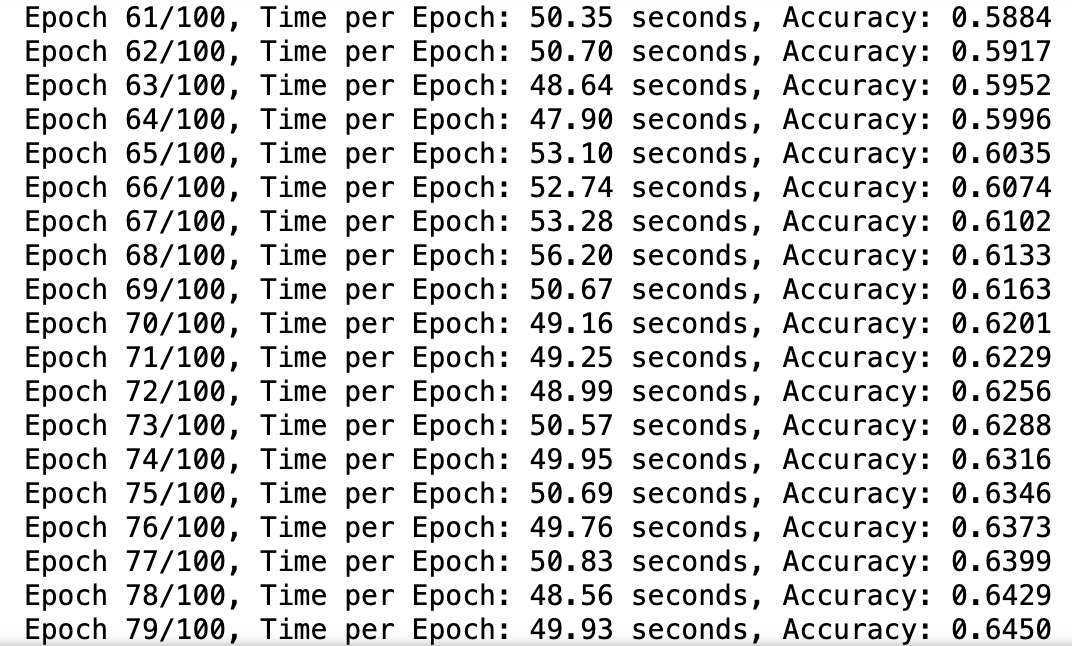
\includegraphics[width=0.6\linewidth, height=3cm]{no_latency.png}
    \caption{FL model accuracy over iterations under normal network conditions.}
    \label{fig:no_latency} 
\end{figure}

\begin{figure}[!ht]
    \centering
    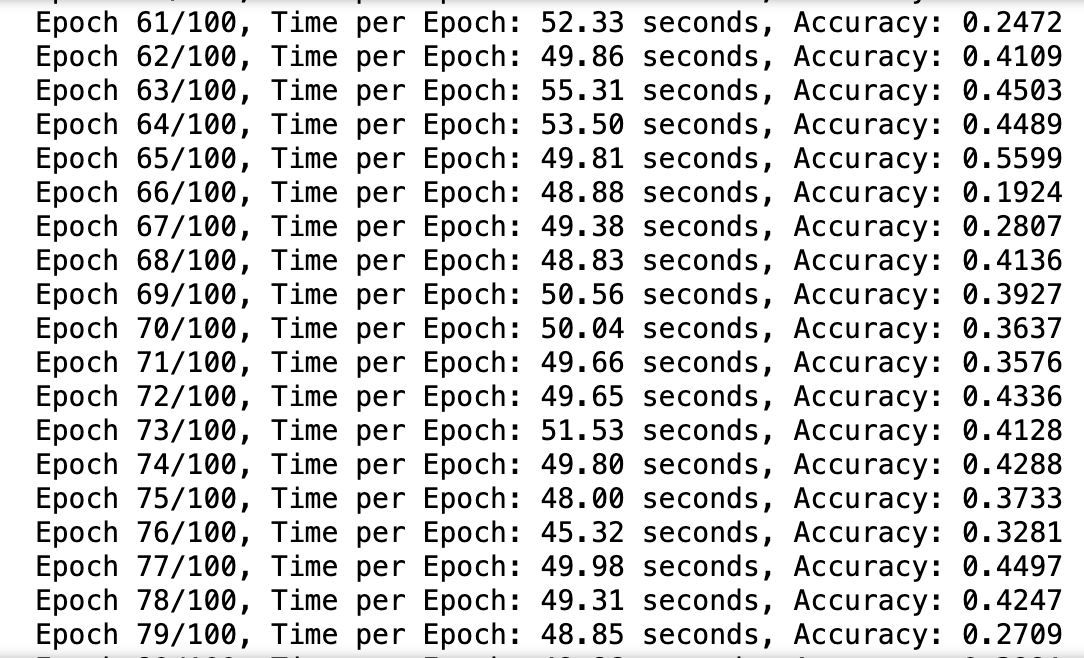
\includegraphics[width=0.6\linewidth, height=3cm]{latency.png}
    \caption{FL model accuracy over iterations under congested network conditions.}
    \label{fig:latency}
\end{figure}

\FloatBarrier

Experimental results also show that although the training process of the model exhibits significant fluctuations under network congestion, with sufficient iterations and an adequate amount of data from each client, the model eventually stabilizes. This final stable state is comparable to the model trained with a sufficient number of iterations under normal network conditions.

\begin{figure}[!ht]
    \centering
    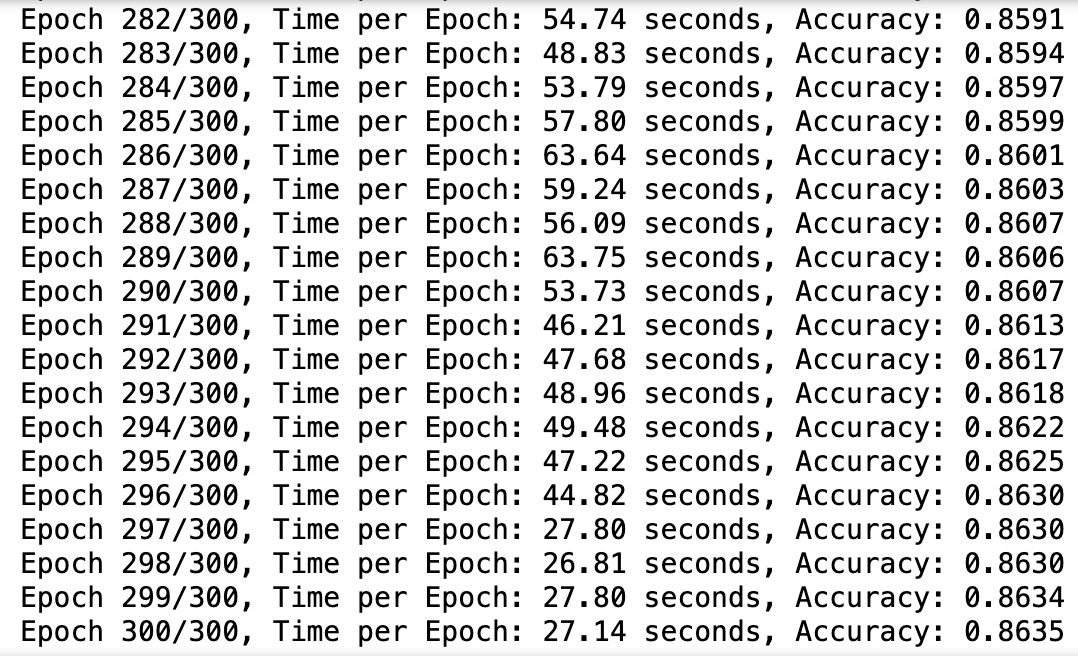
\includegraphics[width=0.6\linewidth, height=3cm]{no_latency_enough_epoch.png}
    \caption{After enough iterations under normal network conditions.}
    \label{fig:no_latency} 
\end{figure}

\begin{figure}[!ht]
    \centering
    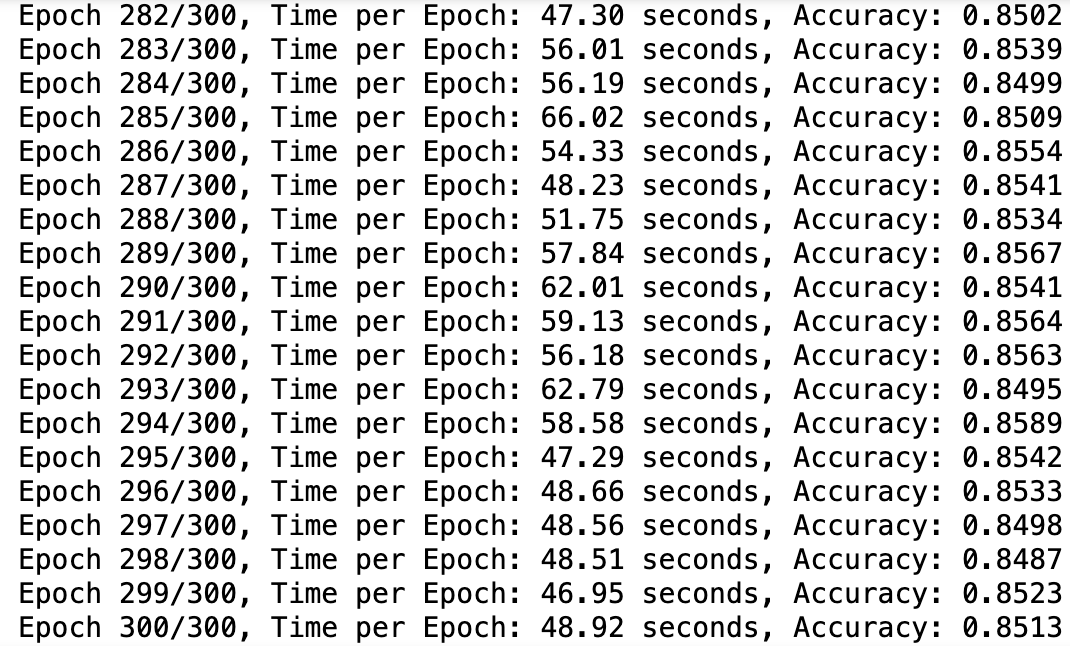
\includegraphics[width=0.6\linewidth, height=3cm]{latency_enough_epoch.png}
    \caption{After enough iterations under congested network conditions.}
    \label{fig:latency}
\end{figure}

\FloatBarrier

\section{Conclusion and Future Work}

In this study, we first measured the latency data from a local machine to remote machines located on the East and West Coasts of the United States using three cloud service platforms: AWS, Google Cloud, and Azure. These measurements were taken under various network congestion conditions such as TCP traffic and UDP traffic. We then applied the latency data to a federated learning model. The study results indicate that network latency significantly impacts the training process of federated learning, causing considerable fluctuations in accuracy on the test set. However, after prolonged training, the final model performance approaches that of the model trained under normal network conditions. Additionally, the threshold set at the central server significantly affects the model's training. To mitigate the impact of network congestion on federated learning, choosing an appropriate threshold is a critical area for further research.


\begin{thebibliography}{00}

\bibitem{b2} Yann LeCun, ``MNIST Handwritten Digit Database,'' 2024. [Online]. Available: \url{http://yann.lecun.com/exdb/mnist/}. [Accessed: May 13, 2024].
%\bibitem{b3} Sanchez-Iborra, R., \& Skarmeta, A. F., ``TinyML-enabled frugal smart objects: Challenges and opportunities,'' \emph{IEEE Circuits and Systems Magazine}, vol. 20, no. 3, pp. 4-18, 2020. [Online]. Available: \url{https://ieeexplore.ieee.org/abstract/document/9166461?casa_token=oQTlhfGuseAAAAAA:YLU6l3Z6Re_-waBbUh-h8nbIhah8zwGJEYUxrP5R9rqCjjYzLdvqbfmAI4-mjhm53jMT8V-g}. [Accessed: May 13, 2024].


\end{thebibliography}


\end{document}
